\documentclass[11pt,a4paper]{report}

% ─── Packages ───
\usepackage[utf8]{inputenc}
\usepackage[T1]{fontenc}
\usepackage[margin=1in, top=1.2in, bottom=1.2in]{geometry}
\usepackage{amsmath,amssymb,amsthm,mathtools}
\usepackage{xcolor}
\usepackage{titlesec}
\usepackage{titletoc}
\usepackage{fancyhdr}
\usepackage{enumitem}
\usepackage{tcolorbox}
\usepackage{booktabs}
\usepackage{graphicx}
\usepackage{hyperref}
\usepackage{cleveref}
\usepackage{tikz}
\usepackage{setspace}
\usepackage{parskip}
\usepackage{caption}
\usepackage{etoolbox}
\usepackage{array}
\usepackage{multirow}

\usetikzlibrary{arrows.meta, positioning, shapes.geometric, calc, decorations.pathmorphing, fit, backgrounds, chains}
\tcbuselibrary{skins,breakable,theorems}

% ─── Colors ───
\definecolor{darkgreen}{HTML}{1b5e20}
\definecolor{accentlime}{HTML}{9ccc65}
\definecolor{deepteal}{HTML}{004d40}
\definecolor{softgold}{HTML}{c8a951}
\definecolor{darkbg}{HTML}{0d1f12}
\definecolor{sectionblue}{HTML}{1a3a5c}
\definecolor{subsecblue}{HTML}{2c5f8a}
\definecolor{defcolor}{HTML}{1565c0}
\definecolor{defbg}{HTML}{e3f2fd}
\definecolor{principlecolor}{HTML}{c62828}
\definecolor{principlebg}{HTML}{ffebee}
\definecolor{mechcolor}{HTML}{2e7d32}
\definecolor{mechbg}{HTML}{e8f5e9}
\definecolor{mathbg}{HTML}{f8f5ee}
\definecolor{notepurple}{HTML}{7b1fa2}
\definecolor{notebg}{HTML}{f3e5f5}
\definecolor{lightgray}{HTML}{f0f0f0}
\definecolor{darkgray}{HTML}{333333}
\definecolor{predcolor}{HTML}{e65100}
\definecolor{predbg}{HTML}{fff3e0}
\definecolor{compcolor}{HTML}{4a148c}
\definecolor{compbg}{HTML}{f3e5f5}
\definecolor{stagecolor}{HTML}{00695c}
\definecolor{stagebg}{HTML}{e0f2f1}

% ─── Hyperref Setup ───
\hypersetup{
    colorlinks=true,
    linkcolor=darkgreen,
    citecolor=darkgreen,
    urlcolor=deepteal,
    bookmarks=true,
    bookmarksnumbered=true,
    pdfauthor={Comprehensive Guide},
    pdftitle={Recurrent Processing Theory (RPT)},
    pdfsubject={Consciousness, Visual Neuroscience, Recurrent Processing},
}

% ─── Header/Footer ───
\pagestyle{fancy}
\fancyhf{}
\fancyhead[L]{\small\color{gray} Recurrent Processing Theory (RPT)}
\fancyhead[R]{\small\color{gray} Comprehensive Reading Material}
\fancyfoot[C]{\thepage}
\renewcommand{\headrulewidth}{0.4pt}
\renewcommand{\footrulewidth}{0pt}

\fancypagestyle{plain}{%
  \fancyhf{}
  \fancyfoot[C]{\thepage}
  \renewcommand{\headrulewidth}{0pt}
}

% ─── Chapter/Section Formatting ───
\titleformat{\chapter}[display]
  {\normalfont\huge\bfseries\color{darkgreen}}
  {\chaptertitlename\ \thechapter}{20pt}{\Huge}
\titlespacing*{\chapter}{0pt}{-20pt}{30pt}

\titleformat{\section}
  {\normalfont\Large\bfseries\color{sectionblue}}
  {\thesection}{1em}{}
\titleformat{\subsection}
  {\normalfont\large\bfseries\color{subsecblue}}
  {\thesubsection}{1em}{}
\titleformat{\subsubsection}
  {\normalfont\normalsize\bfseries\color{darkgray}}
  {\thesubsubsection}{1em}{}

% ─── Tcolorbox environments ───
\newtcolorbox{principlebox}[1][]{
  enhanced, breakable,
  colback=principlebg, colframe=principlecolor,
  coltitle=white, fonttitle=\bfseries,
  title=#1,
  left=8pt, right=8pt, top=6pt, bottom=6pt,
  boxrule=0.5pt, arc=3pt,
  borderline west={3pt}{0pt}{principlecolor},
  before skip=10pt, after skip=10pt,
}

\newtcolorbox{mechbox}[1][]{
  enhanced, breakable,
  colback=mechbg, colframe=mechcolor,
  coltitle=white, fonttitle=\bfseries,
  title=#1,
  left=8pt, right=8pt, top=6pt, bottom=6pt,
  boxrule=0.5pt, arc=3pt,
  borderline west={3pt}{0pt}{mechcolor},
  before skip=10pt, after skip=10pt,
}

\newtcolorbox{definitionbox}[1][]{
  enhanced, breakable,
  colback=defbg, colframe=defcolor,
  coltitle=white, fonttitle=\bfseries,
  title=#1,
  left=8pt, right=8pt, top=6pt, bottom=6pt,
  boxrule=0.5pt, arc=3pt,
  borderline west={3pt}{0pt}{defcolor},
  before skip=10pt, after skip=10pt,
}

\newtcolorbox{mathbox}{
  enhanced,
  colback=mathbg, colframe=mathbg!70!black,
  left=8pt, right=8pt, top=6pt, bottom=6pt,
  boxrule=0.3pt, arc=2pt,
  before skip=8pt, after skip=8pt,
}

\newtcolorbox{notebox}[1][Note]{
  enhanced, breakable,
  colback=notebg, colframe=notepurple,
  coltitle=white, fonttitle=\bfseries,
  title=#1,
  left=8pt, right=8pt, top=6pt, bottom=6pt,
  boxrule=0.5pt, arc=3pt,
  borderline west={3pt}{0pt}{notepurple},
  before skip=10pt, after skip=10pt,
}

\newtcolorbox{predbox}[1][]{
  enhanced, breakable,
  colback=predbg, colframe=predcolor,
  coltitle=white, fonttitle=\bfseries,
  title=#1,
  left=8pt, right=8pt, top=6pt, bottom=6pt,
  boxrule=0.5pt, arc=3pt,
  borderline west={3pt}{0pt}{predcolor},
  before skip=10pt, after skip=10pt,
}

\newtcolorbox{compbox}[1][]{
  enhanced, breakable,
  colback=compbg, colframe=compcolor,
  coltitle=white, fonttitle=\bfseries,
  title=#1,
  left=8pt, right=8pt, top=6pt, bottom=6pt,
  boxrule=0.5pt, arc=3pt,
  borderline west={3pt}{0pt}{compcolor},
  before skip=10pt, after skip=10pt,
}

\newtcolorbox{stagebox}[1][]{
  enhanced, breakable,
  colback=stagebg, colframe=stagecolor,
  coltitle=white, fonttitle=\bfseries,
  title=#1,
  left=8pt, right=8pt, top=6pt, bottom=6pt,
  boxrule=0.5pt, arc=3pt,
  borderline west={3pt}{0pt}{stagecolor},
  before skip=10pt, after skip=10pt,
}

\newtcolorbox{examplebox}[1][Example]{
  enhanced, breakable,
  colback=lightgray, colframe=darkgreen!60,
  coltitle=white, fonttitle=\bfseries,
  title=#1,
  left=8pt, right=8pt, top=6pt, bottom=6pt,
  boxrule=0.5pt, arc=3pt,
  before skip=10pt, after skip=10pt,
}

\setlength{\parindent}{0pt}
\setlength{\parskip}{6pt}

% ══════════════════════════════════════════════════════════════
\begin{document}

% ─── COVER PAGE ───
\begin{titlepage}
\begin{tikzpicture}[remember picture, overlay]
  % Background
  \fill[darkbg] (current page.south west) rectangle (current page.north east);
  % Accent line
  \fill[accentlime] ([yshift=-11cm]current page.north west) rectangle ([yshift=-10.85cm]current page.north east);
  % Decorative recurrent loops
  \foreach \x/\y/\s in {3/-13/0.6, 6/-14/0.8, 9/-12.5/0.5, 4.5/-15.5/0.7, 7.5/-15/0.55} {
    \draw[accentlime, opacity=0.12, line width=0.6pt, ->] (\x,\y) arc[start angle=0, end angle=320, radius=\s];
  }
  % Feedforward arrows
  \foreach \y in {-12, -13.5, -15} {
    \draw[white, opacity=0.04, line width=2pt, -Stealth] (2, \y) -- (10, \y);
  }
  % Feedback arrows
  \foreach \y in {-12.7, -14.2} {
    \draw[accentlime, opacity=0.06, line width=1.5pt, -Stealth, dashed] (10, \y) -- (2, \y);
  }
  % Large symbol
  \node[text=accentlime, opacity=0.05, scale=16] at ([yshift=-4cm, xshift=5cm]current page.center) {\textbf{RP}};
\end{tikzpicture}

\vspace*{4cm}
\begin{center}
  {\fontsize{34}{42}\selectfont\bfseries\color{white} Recurrent Processing\\[8pt] Theory (RPT)}\\[24pt]
  {\Large\color{gray!70} A Comprehensive Mathematical \& Conceptual Guide}\\[20pt]
  {\color{accentlime}\rule{6cm}{1pt}}\\[20pt]
  {\large\color{gray!60} Feedforward vs.\ Recurrent Processing:\\[4pt] How Feedback Loops Give Rise to Visual Awareness}\\[40pt]
  {\color{softgold}\large Victor A.\ F.\ Lamme}\\[8pt]
  {\color{gray!50}\normalsize Prerequisites $\bullet$ Processing Stages $\bullet$ Neural Mechanisms $\bullet$ Formal Models}\\[60pt]
  {\color{gray!40}\small Comprehensive Study Material \quad$\vert$\quad February 2026}
\end{center}
\end{titlepage}

% ─── TABLE OF CONTENTS ───
\tableofcontents
\thispagestyle{plain}
\newpage


% ══════════════════════════════════════════════════════════════
\chapter{Introduction to Recurrent Processing Theory}
% ══════════════════════════════════════════════════════════════

\section{What is Recurrent Processing Theory?}

Recurrent Processing Theory (RPT) is a neuroscientific theory of visual consciousness developed primarily by \textbf{Victor A.\ F.\ Lamme}, a neuroscientist at the University of Amsterdam, beginning in the early 2000s. RPT proposes that conscious visual experience does not arise from the initial feedforward sweep of neural activity through the visual hierarchy, but rather from \textbf{recurrent (feedback) processing}---the re-entrant signals that flow \emph{backward} from higher to lower cortical areas.

\begin{definitionbox}[Core Claim of RPT]
Consciousness requires \textbf{recurrent processing} within sensory cortex. The initial feedforward sweep of activity through the visual hierarchy is necessary but not sufficient for awareness. It is only when higher-level areas send feedback signals back to earlier areas, creating recurrent loops, that visual experience arises. Crucially, this recurrent processing in \emph{sensory cortex itself} may suffice---prefrontal cortex involvement is not necessary for phenomenal consciousness.
\end{definitionbox}

\section{Historical Context and Motivation}

RPT emerged from a confluence of findings in visual neuroscience:

\textbf{(a) Feedforward vs.\ feedback in visual cortex:} By the 1990s, it was well established that visual processing involves not only a ``feedforward'' sweep from retina $\to$ LGN $\to$ V1 $\to$ V2 $\to$ V4 $\to$ IT, but also massive \textbf{feedback} (recurrent) connections from higher areas back to lower areas. In fact, feedback connections outnumber feedforward connections in most cortical areas.

\textbf{(b) The timing of visual awareness:} Lamme and Roelfsema (2000) showed that neural responses in V1 have two distinct phases: an early component ($\sim$40--80 ms) reflecting feedforward processing, and a later component ($\sim$80--200 ms) reflecting feedback from higher areas. Crucially, the late feedback-driven component correlates with visual awareness, while the early feedforward component does not.

\textbf{(c) Masking and the disruption of recurrence:} Visual masking experiments showed that a mask presented shortly after a target disrupts awareness of the target, even though the feedforward response to the target in V1 is largely intact. This suggests that masking works by disrupting the \emph{recurrent} processing that is necessary for awareness.

\textbf{(d) Dissatisfaction with prefrontal theories:} Lamme was critical of theories like GNWT that require prefrontal cortex for consciousness. He argued that the phenomenological richness of visual experience far exceeds what could be maintained in a capacity-limited prefrontal workspace, and that sensory cortex itself has the computational resources to generate consciousness.

\section{RPT's Stance on the Hard Problem}

RPT is primarily a theory about the \textbf{neural mechanisms} of consciousness, particularly visual consciousness. It does not claim to solve the Hard Problem directly. However, Lamme argues that once we correctly identify the neural mechanisms (recurrent processing), the Hard Problem becomes more tractable---or at least, we know where to look for its solution.

Lamme's position is that phenomenal consciousness should be identified with the recurrent processing itself, not with the \emph{reports} about that processing. This has important implications: a system could be phenomenally conscious (have experiences) without being able to report on them---a claim that puts RPT in tension with both GWT and some interpretations of IIT.

\section{Overview of the Framework}

RPT organizes visual processing into a hierarchy of stages, each associated with a different level of consciousness:

\begin{enumerate}[leftmargin=2em]
  \item \textbf{Stage 1 --- Feedforward sweep:} Fast, automatic, unconscious processing propagating from lower to higher areas.
  \item \textbf{Stage 2 --- Local recurrent processing:} Feedback within and between sensory areas, giving rise to phenomenal consciousness without reportability.
  \item \textbf{Stage 3 --- Global recurrent processing:} Feedback involving prefrontal and parietal areas, enabling reportable, access-conscious states.
\end{enumerate}

The controversial claim of RPT is that Stage 2 is already \emph{conscious}---phenomenal experience exists in the recurrent loops of sensory cortex alone, even without prefrontal involvement.


% ══════════════════════════════════════════════════════════════
\chapter{Mathematical and Neuroscientific Prerequisites}
% ══════════════════════════════════════════════════════════════

\section{Visual Cortex Anatomy}

Understanding RPT requires a grasp of the hierarchical organization of visual cortex and its connectivity.

\subsection{The Visual Hierarchy}

The primate visual system is organized as a rough hierarchy:

\begin{center}
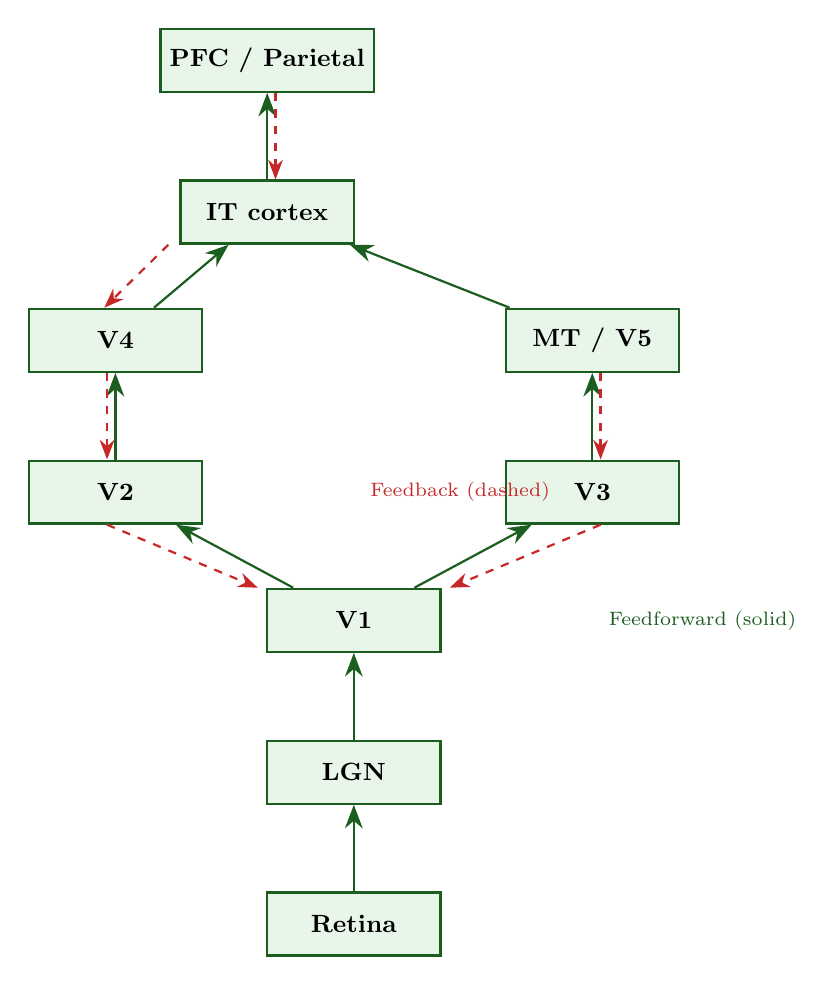
\begin{tikzpicture}[
    box/.style={rectangle, draw=darkgreen, fill=mechbg, thick, minimum width=2.2cm, minimum height=0.8cm, font=\small\bfseries, align=center},
    ff/.style={-{Stealth[length=3mm]}, thick, darkgreen},
    fb/.style={-{Stealth[length=2.5mm]}, thick, principlecolor, dashed},
    node distance=1.1cm,
  ]
  \node[box] (ret) {Retina};
  \node[box, above=of ret] (lgn) {LGN};
  \node[box, above=of lgn] (v1) {V1};
  \node[box, above left=0.8cm and 0.8cm of v1] (v2) {V2};
  \node[box, above right=0.8cm and 0.8cm of v1] (v3) {V3};
  \node[box, above=of v2] (v4) {V4};
  \node[box, above=of v3] (mt) {MT / V5};
  \node[box, above right=0.8cm and -0.3cm of v4] (it) {IT cortex};
  \node[box, above=of it] (pfc) {PFC / Parietal};

  % Feedforward
  \draw[ff] (ret) -- (lgn);
  \draw[ff] (lgn) -- (v1);
  \draw[ff] (v1) -- (v2);
  \draw[ff] (v1) -- (v3);
  \draw[ff] (v2) -- (v4);
  \draw[ff] (v3) -- (mt);
  \draw[ff] (v4) -- (it);
  \draw[ff] (mt) -- (it);
  \draw[ff] (it) -- (pfc);

  % Feedback (dashed, red)
  \draw[fb] ([xshift=-3pt]v2.south) -- ([xshift=-3pt]v1.north west);
  \draw[fb] ([xshift=3pt]v3.south) -- ([xshift=3pt]v1.north east);
  \draw[fb] ([xshift=-3pt]v4.south) -- ([xshift=-3pt]v2.north);
  \draw[fb] ([xshift=3pt]mt.south) -- ([xshift=3pt]v3.north);
  \draw[fb] ([xshift=-4pt]it.south west) -- ([xshift=-4pt]v4.north);
  \draw[fb] ([xshift=3pt]pfc.south) -- ([xshift=3pt]it.north);

  % Labels
  \node[right=2cm of v1, font=\scriptsize\color{darkgreen}] {Feedforward (solid)};
  \node[right=2cm of v2, font=\scriptsize\color{principlecolor}] {Feedback (dashed)};
\end{tikzpicture}
\end{center}
\vspace{-2pt}
{\small\centering\textit{Figure: The visual hierarchy with feedforward (solid green) and feedback (dashed red) connections.}\par}

Key anatomical facts:
\begin{itemize}[leftmargin=1.5em]
  \item Feedforward connections originate primarily from layer 2/3 neurons and terminate in layer 4.
  \item Feedback connections originate from layers 5/6 and deep layer 2/3, terminating in layers 1 and 5/6.
  \item Feedback connections are \textbf{more numerous} than feedforward connections in most areas.
  \item Lateral connections within a cortical area (horizontal connections in layer 2/3) provide a third type of connectivity.
\end{itemize}

\subsection{Receptive Field Properties}

\begin{definitionbox}[Classical vs.\ Extra-Classical Receptive Field]
\begin{itemize}[leftmargin=1.5em]
  \item The \textbf{classical receptive field} (CRF) of a neuron is the region of visual space where stimuli directly drive the neuron's response. CRF properties are largely determined by \emph{feedforward} input.
  \item The \textbf{extra-classical receptive field} (eCRF) or surround refers to modulation of the neuron's response by stimuli outside the CRF. These modulations are driven largely by \emph{feedback} and \emph{lateral} connections.
\end{itemize}
The key RPT insight: early CRF responses ($\sim$40--60 ms) reflect feedforward processing; later eCRF modulations ($\sim$80--200 ms) reflect recurrent processing and correlate with awareness.
\end{definitionbox}

\section{Dynamics of Cortical Circuits}

\subsection{Excitatory--Inhibitory Balance}

Cortical circuits maintain a balance between excitation (E) and inhibition (I). The E/I dynamics are critical for understanding both feedforward propagation and recurrent amplification.

\begin{mathbox}
\vspace{-6pt}
\begin{align}
  \tau_E \frac{dE_l}{dt} &= -E_l + f\!\left(w_{EE}^{l} E_l - w_{EI}^{l} I_l + w_{FF}^{l} E_{l-1} + w_{FB}^{l} E_{l+1} + I_{\text{ext}}^l\right) \label{eq:exc} \\[6pt]
  \tau_I \frac{dI_l}{dt} &= -I_l + f\!\left(w_{IE}^{l} E_l - w_{II}^{l} I_l\right) \label{eq:inh}
\end{align}
\vspace{-8pt}
\end{mathbox}

where $l$ indexes the cortical layer/area, $w_{FF}^l$ is the feedforward weight from layer $l{-}1$, $w_{FB}^l$ is the feedback weight from layer $l{+}1$, and $f(\cdot)$ is a sigmoidal or threshold-linear activation function. In RPT, the critical term is $w_{FB}^l E_{l+1}$---the feedback signal that creates recurrent processing.

\subsection{Laminar Circuitry}

Feedback connections have distinct laminar targets compared to feedforward:

\begin{center}
\renewcommand{\arraystretch}{1.3}
\begin{tabular}{>{\raggedright}p{3.5cm} >{\raggedright}p{4.5cm} >{\raggedright\arraybackslash}p{4.5cm}}
  \toprule
  \textbf{Property} & \textbf{Feedforward} & \textbf{Feedback} \\
  \midrule
  Origin layers & Superficial (2/3) & Deep (5/6) and superficial \\
  Target layers & Layer 4 (granular) & Layers 1, 5/6 (agranular) \\
  Latency & Short ($\sim$10 ms/synapse) & Slightly longer \\
  Spatial extent & Focused, topographic & Diffuse, modulatory \\
  Neurotransmitter effect & Driving (strong AMPA) & Modulatory (NMDA-rich) \\
  \bottomrule
\end{tabular}
\end{center}

The fact that feedback connections are \textbf{NMDA-receptor-rich} is significant: NMDA receptors are voltage-dependent and have slow kinetics, making feedback connections ideally suited for sustained, modulatory (rather than driving) effects. This also makes recurrent processing sensitive to NMDA-receptor antagonists (e.g., ketamine).

\section{Neural Oscillations and Communication}

Recurrent processing involves specific oscillatory signatures. Understanding these requires basic concepts from signal analysis.

\subsection{Neural Oscillations: Frequency Bands}

\begin{definitionbox}[Cortical Oscillation Bands]
\begin{itemize}[leftmargin=1.5em]
  \item \textbf{Alpha} ($8$--$13$ Hz): Associated with cortical inhibition and gating.
  \item \textbf{Beta} ($13$--$30$ Hz): Linked to feedback signaling and top-down processing.
  \item \textbf{Gamma} ($30$--$100$ Hz): Linked to feedforward signaling and local processing.
  \item \textbf{Theta} ($4$--$8$ Hz): Involved in memory and long-range coordination.
\end{itemize}
RPT-relevant finding: \textbf{feedforward} processing is associated with \textbf{gamma-band} activity, while \textbf{feedback} processing is associated with \textbf{alpha/beta-band} activity. These operate in different cortical layers.
\end{definitionbox}

\subsection{Spectral Granger Causality}

To quantify directed information flow in specific frequency bands, we use \textbf{spectral Granger causality}:

\begin{mathbox}
\vspace{-8pt}
\[
  \mathcal{G}_{X \to Y}(\omega) = \ln \frac{S_{YY}(\omega)}{S_{YY}(\omega) - \frac{|\Sigma_{12}|^2}{\Sigma_{11}} |H_{Y|X}(\omega)|^2}
\]
\vspace{-10pt}
\end{mathbox}

where $S_{YY}(\omega)$ is the power spectral density of $Y$, $H_{Y|X}(\omega)$ is the transfer function from $X$ to $Y$, and $\Sigma$ is the noise covariance matrix from the vector autoregressive (VAR) model:
\begin{align}
  X_t &= \sum_{k=1}^{p} a_{11}^{(k)} X_{t-k} + \sum_{k=1}^{p} a_{12}^{(k)} Y_{t-k} + \varepsilon_{1,t} \\
  Y_t &= \sum_{k=1}^{p} a_{21}^{(k)} X_{t-k} + \sum_{k=1}^{p} a_{22}^{(k)} Y_{t-k} + \varepsilon_{2,t}
\end{align}

In RPT research, spectral Granger causality is used to demonstrate that feedforward information flow (V1 $\to$ V4) is carried in the \textbf{gamma band}, while feedback flow (V4 $\to$ V1) is carried in the \textbf{alpha/beta band}---and that awareness correlates specifically with the feedback component.

\section{Predictive Coding Framework}

RPT has deep connections to \textbf{predictive coding}, which provides a computational rationale for feedback connections.

\begin{definitionbox}[Predictive Coding]
In predictive coding, each level $l$ of the cortical hierarchy maintains a generative model that \emph{predicts} the activity of the level below. Feedback connections carry \textbf{predictions} (top-down priors), while feedforward connections carry \textbf{prediction errors} (the discrepancy between prediction and actual input):
\begin{align}
  \text{Prediction error:}\quad \varepsilon_l &= x_l - g_l(\hat{x}_{l+1}) \label{eq:pe} \\[4pt]
  \text{State update:}\quad \dot{\hat{x}}_{l+1} &= -\frac{\partial}{\partial \hat{x}_{l+1}} F = \underbrace{D\hat{x}_{l+1}}_{\text{prior dynamics}} - \underbrace{\frac{\partial g_l^T}{\partial \hat{x}_{l+1}} \Pi_l\, \varepsilon_l}_{\text{error correction}} \label{eq:update}
\end{align}
where $g_l$ is the generative model at level $l$, $\hat{x}_{l+1}$ is the top-down prediction, $\Pi_l$ is the precision (inverse variance) of the prediction error, and $F$ is the variational free energy.
\end{definitionbox}

In this framework, recurrent processing is the iterative exchange of predictions (feedback) and prediction errors (feedforward) that settles into a stable percept. RPT can be understood as claiming that this iterative settling process, when it occurs within sensory cortex, \emph{is} phenomenal consciousness.


% ══════════════════════════════════════════════════════════════
\chapter{The Three Stages of Visual Processing}
% ══════════════════════════════════════════════════════════════

RPT's most distinctive contribution is its taxonomy of visual processing into three stages, each with distinct neural mechanisms and different relationships to consciousness.

\section{Stage 1: The Feedforward Sweep}

\begin{stagebox}[Stage 1 --- Feedforward Sweep (Unconscious)]
The initial wave of neural activity propagating from retina through LGN to V1, then through the ventral (``what'') and dorsal (``where/how'') streams. This sweep is \textbf{fast} ($\sim$40--100 ms to reach IT cortex), \textbf{automatic}, and \textbf{unconscious}. It extracts basic visual features and even high-level categorical information (e.g., ``is this a face or a house?''), but does not produce awareness.
\end{stagebox}

\subsection{Properties of the Feedforward Sweep}

\begin{enumerate}[leftmargin=2em]
  \item \textbf{Speed:} The feedforward sweep propagates at approximately 10 ms per synapse, reaching V1 at $\sim$40 ms, V4 at $\sim$60 ms, and IT cortex at $\sim$80--100 ms after stimulus onset.
  \item \textbf{Hierarchical feature extraction:} V1 encodes oriented edges, V2 encodes texture boundaries, V4 encodes shape and color, and IT encodes object categories. Each level extracts progressively more complex features.
  \item \textbf{No awareness:} Despite extracting rich information, the feedforward sweep does not produce conscious perception. Evidence: stimuli that are masked before recurrent processing can occur are not consciously seen, even though they activate IT cortex in the feedforward sweep.
  \item \textbf{Behavioral influence:} Although unconscious, feedforward processing can influence behavior (e.g., priming, fast motor responses, subliminal categorization).
\end{enumerate}

\subsection{Mathematical Model of Feedforward Processing}

A simple model of the feedforward sweep through $L$ hierarchical layers:

\begin{mathbox}
\vspace{-6pt}
\begin{align}
  \mathbf{r}_l(t) &= f\!\left(W_l^{FF}\, \mathbf{r}_{l-1}(t - \delta_l) + \mathbf{b}_l\right), \qquad l = 1, 2, \ldots, L \label{eq:ff_model}\\[6pt]
  \mathbf{r}_0(t) &= \mathbf{s}(t) \quad \text{(stimulus input)}
\end{align}
\vspace{-8pt}
\end{mathbox}

where $\mathbf{r}_l(t)$ is the population activity vector at level $l$, $W_l^{FF}$ is the feedforward weight matrix, $\delta_l$ is the propagation delay, $\mathbf{b}_l$ is a bias, and $f(\cdot)$ is a nonlinear activation (e.g., ReLU or sigmoid). This model is essentially a \textbf{deep feedforward neural network}, and Lamme notes that such networks, however sophisticated, are not conscious according to RPT.

\subsection{Evidence for Unconscious Feedforward Processing}

Key experiments demonstrating sophisticated unconscious feedforward processing:

\begin{examplebox}[Ultra-Rapid Categorization (Thorpe et al., 1996)]
Subjects can categorize natural images (animal vs.\ non-animal) in as little as $\sim$150 ms, with differential ERP responses as early as $\sim$150 ms. The earliest category-selective signals occur before recurrent processing has had time to develop, suggesting feedforward processing can extract categorical information unconsciously.
\end{examplebox}

\begin{examplebox}[Masked Priming in IT Cortex (Rolls \& Tovee, 1994)]
Neurons in IT cortex respond selectively to masked faces that subjects cannot consciously perceive. The feedforward response is present but short-lived; without recurrent amplification, the signal fades and awareness does not occur.
\end{examplebox}

\section{Stage 2: Local Recurrent Processing}

\begin{stagebox}[Stage 2 --- Local Recurrent Processing (Phenomenal Consciousness)]
Beginning $\sim$80--120 ms after stimulus onset, feedback signals from higher visual areas (V4, IT) arrive back at lower areas (V1, V2), creating \textbf{recurrent loops} within the visual cortex. This local recurrent processing gives rise to \textbf{phenomenal consciousness}---the subjective visual experience---even without prefrontal involvement. This stage is \textbf{capacity-rich} but \textbf{not reportable} without further (Stage 3) processing.
\end{stagebox}

This is the most controversial and distinctive claim of RPT.

\subsection{Properties of Local Recurrent Processing}

\begin{enumerate}[leftmargin=2em]
  \item \textbf{Feedback modulation:} Higher areas send predictions and contextual information back to lower areas, modulating the feedforward response. This creates figure-ground segregation, texture segmentation, contour integration, and other perceptual grouping phenomena.
  \item \textbf{Amplification:} Recurrent processing amplifies and sustains the neural representation, making it robust against noise and masking.
  \item \textbf{Feature binding:} Recurrent processing binds features across different cortical areas into a unified percept (e.g., the color and shape of an object).
  \item \textbf{Phenomenal consciousness:} According to RPT, the recurrent interaction between visual areas creates phenomenal experience. The rich, detailed visual world we experience reflects the capacity of recurrent sensory processing.
  \item \textbf{No reportability (yet):} At this stage, the experience exists but is not yet available for verbal report, working memory, or deliberate action. It is ``phenomenally conscious'' but not ``access conscious'' (in Ned Block's terminology).
\end{enumerate}

\subsection{Mathematical Model: Recurrent Amplification}

Adding feedback to the feedforward model:

\begin{mathbox}
\vspace{-6pt}
\begin{align}
  \tau_l \frac{d\mathbf{r}_l}{dt} &= -\mathbf{r}_l + f\!\left(\underbrace{W_l^{FF}\, \mathbf{r}_{l-1}}_{\text{feedforward}} + \underbrace{W_l^{FB}\, \mathbf{r}_{l+1}}_{\text{feedback}} + \underbrace{W_l^{LAT}\, \mathbf{r}_{l}}_{\text{lateral}} + \mathbf{b}_l\right) \label{eq:recurrent_model}
\end{align}
\vspace{-8pt}
\end{mathbox}

The feedback term $W_l^{FB}\, \mathbf{r}_{l+1}$ is the key addition. This creates a dynamical system that, instead of settling in one feedforward pass, iterates toward a stable attractor through multiple cycles of feedforward--feedback exchange.

\textbf{Recurrent amplification} can be analyzed through the effective gain. Consider a simplified one-dimensional version with feedforward input $x$ and recurrent weight $w_r$:
\[
  r = f(x + w_r \cdot r)
\]
For a linear approximation ($f(u) \approx u$ near the fixed point):
\[
  r = \frac{x}{1 - w_r} \qquad \text{(provided } w_r < 1\text{)}
\]

The effective gain is $G = 1/(1 - w_r)$, which diverges as $w_r \to 1$. Recurrent connectivity amplifies the input signal by a factor that depends on the strength of feedback. When $w_r$ is strong, even weak inputs are amplified into robust, sustained representations.

\subsection{Figure-Ground Segregation: A Paradigmatic Example}

Lamme's foundational experiments on \textbf{figure-ground segregation} in V1 of macaque monkeys provide the clearest demonstration of recurrent processing:

\begin{examplebox}[Figure-Ground Modulation in V1 (Lamme, 1995)]
When a textured figure is presented on a textured background, V1 neurons whose receptive fields fall on the figure show enhanced responses compared to neurons responding to the background. However:
\begin{itemize}[leftmargin=1.5em]
  \item The \textbf{initial response} (40--60 ms) is identical for figure and background (feedforward).
  \item The \textbf{figure-ground modulation} appears at $\sim$80--100 ms, reflecting feedback from higher areas (V4, IT) that have computed the figure-ground boundary.
  \item This modulation is \textbf{abolished by anesthesia} (which disrupts recurrent processing) while the initial response is preserved.
  \item The modulation correlates with the monkey's \textbf{behavioral detection} of the figure.
\end{itemize}
\end{examplebox}

This experiment elegantly dissociates feedforward (unconscious) from recurrent (conscious-linked) processing in the same neurons.

\section{Stage 3: Global Recurrent Processing}

\begin{stagebox}[Stage 3 --- Global Recurrent Processing (Access Consciousness)]
When the recurrent activity in sensory cortex is strong enough and sufficiently sustained, it propagates to \textbf{prefrontal} and \textbf{parietal} cortex, engaging a broader network. This global recurrent processing enables \textbf{access consciousness}: the ability to report, remember, and deliberately act on the perceived information. This stage is \textbf{capacity-limited} and involves attention and working memory.
\end{stagebox}

\subsection{Relationship to GWT}

Stage 3 of RPT is essentially equivalent to what GWT describes as ``global workspace ignition.'' The key difference is that RPT treats Stage 3 as providing \emph{access} to an experience that already exists at Stage 2, while GWT treats Stage 3 as the \emph{only} form of consciousness.

\subsection{Properties of Global Recurrent Processing}

\begin{enumerate}[leftmargin=2em]
  \item \textbf{Capacity-limited:} Unlike the rich phenomenal experience of Stage 2, Stage 3 can only handle a few items at a time (the working memory bottleneck).
  \item \textbf{Attention-dependent:} Requires top-down attentional selection to route information from sensory cortex to prefrontal/parietal areas.
  \item \textbf{Reportable:} Information at this stage can be verbally reported, used for decision-making, and encoded into long-term memory.
  \item \textbf{Associated with P3b:} The electrophysiological signature of Stage 3 is the P3b wave ($\sim$300--500 ms), consistent with GNWT's ignition marker.
\end{enumerate}

\section{Summary: The Three-Stage Model}

\begin{center}
\renewcommand{\arraystretch}{1.4}
\begin{tabular}{>{\raggedright}p{2.8cm} >{\centering}p{3cm} >{\centering}p{3cm} >{\centering\arraybackslash}p{3.5cm}}
  \toprule
  & \textbf{Stage 1} & \textbf{Stage 2} & \textbf{Stage 3} \\
  \midrule
  \textbf{Processing type} & Feedforward & Local recurrent & Global recurrent \\
  \textbf{Timing} & 40--100 ms & 80--200 ms & 200--500 ms \\
  \textbf{Brain areas} & Sensory hierarchy & Within sensory cortex & Sensory + PFC + parietal \\
  \textbf{Consciousness} & None & \textcolor{mechcolor}{\textbf{Phenomenal}} & \textcolor{defcolor}{\textbf{Access}} \\
  \textbf{Capacity} & Unlimited & Rich, detailed & Limited (3--4 items) \\
  \textbf{Reportability} & No & No & Yes \\
  \textbf{Masking effect} & Preserved & Disrupted & Disrupted \\
  \textbf{Anesthesia} & Preserved & Disrupted & Disrupted \\
  \bottomrule
\end{tabular}
\end{center}


% ══════════════════════════════════════════════════════════════
\chapter{Neural Mechanisms of Recurrent Processing}
% ══════════════════════════════════════════════════════════════

\section{Feedback Connections: Anatomy and Physiology}

\subsection{Anatomical Properties}

Feedback connections in the visual cortex have several distinctive properties:

\begin{mechbox}[Feedback Connection Properties]
\begin{enumerate}[leftmargin=1.5em]
  \item \textbf{Diffuse termination:} Feedback connections terminate diffusely in layers 1 and 5/6, contacting the apical dendrites of pyramidal neurons in layer 2/3. This suggests a \emph{modulatory} rather than \emph{driving} role.
  \item \textbf{Broad spatial extent:} A single feedback projection from V4 can modulate a region of V1 corresponding to a large portion of the visual field, explaining contextual surround effects.
  \item \textbf{NMDA-receptor enrichment:} Feedback synapses preferentially activate NMDA receptors, which are voltage-dependent and have slow kinetics ($\tau_{\text{NMDA}} \sim 50$--$150$ ms vs.\ $\tau_{\text{AMPA}} \sim 2$--$10$ ms).
  \item \textbf{Numerical dominance:} In most cortical areas, feedback connections outnumber feedforward connections by a factor of $\sim$10:1.
\end{enumerate}
\end{mechbox}

\subsection{NMDA-Dependent Recurrence}

The NMDA receptor's voltage dependence creates a natural \textbf{gating mechanism} for recurrence:

\begin{mathbox}
\vspace{-6pt}
\[
  I_{\text{NMDA}}(V, t) = g_{\text{NMDA}}\, s(t)\, B(V)\, (V - E_{\text{syn}})
\]
where the voltage-dependent magnesium block is:
\[
  B(V) = \frac{1}{1 + \frac{[\text{Mg}^{2+}]}{3.57}\, e^{-0.062\, V}}
\]
\vspace{-8pt}
\end{mathbox}

The function $B(V)$ is near zero at resting potential ($V \approx -70$ mV) and rises sharply as the neuron is depolarized. This means NMDA-mediated feedback is only effective when the postsynaptic neuron is \emph{already active} (depolarized by feedforward input). This creates a coincidence detection mechanism: feedback only amplifies neurons that received feedforward input, preventing runaway excitation.

\begin{notebox}[NMDA and Anesthesia]
Many general anesthetics (e.g., ketamine, nitrous oxide) are NMDA receptor antagonists. According to RPT, this is why they abolish consciousness: by blocking NMDA receptors, they selectively disrupt recurrent processing while leaving feedforward processing (mediated by AMPA receptors) largely intact. This provides a pharmacological dissociation between feedforward and recurrent processing.
\end{notebox}

\section{Temporal Dynamics of Recurrence}

\subsection{Two Phases of the V1 Response}

Lamme and colleagues (2000, 2004) demonstrated that V1 neurons show two distinct response phases:

\begin{enumerate}[leftmargin=2em]
  \item \textbf{Early phase} ($\sim$40--80 ms): Driven by feedforward input. Reflects classical receptive field properties (orientation, spatial frequency). NOT correlated with awareness.
  \item \textbf{Late phase} ($\sim$80--250 ms): Driven by recurrent feedback from V2, V4, IT. Reflects contextual modulation (figure-ground, texture segregation, contour integration). CORRELATED with awareness.
\end{enumerate}

Mathematically, the response of a V1 neuron to a stimulus can be decomposed:

\begin{mathbox}
\vspace{-6pt}
\[
  r(t) = \underbrace{r_{\text{FF}}(t)}_{\text{feedforward}} + \underbrace{r_{\text{FB}}(t)}_{\text{feedback}} = \sum_{k} w_k^{FF}\, s_k(t - \delta_{\text{FF}}) \;+\; \sum_{j} w_j^{FB}\, a_j(t - \delta_{\text{FB}})
\]
\vspace{-8pt}
\end{mathbox}

where $s_k$ are feedforward inputs (with delay $\delta_{\text{FF}} \approx 40$ ms) and $a_j$ are feedback signals from higher areas (with delay $\delta_{\text{FB}} \approx 80$--$100$ ms).

\subsection{The ``Recurrent Window'' and Masking}

Visual masking disrupts awareness by interrupting recurrent processing. A mask presented at stimulus-onset asynchrony (SOA) of $\sim$30--80 ms after the target arrives in V1 just as the feedback signals would be returning, effectively overwriting them:

\begin{mathbox}
\vspace{-6pt}
The target representation at time $t$ in V1:
\[
  r_{\text{target}}(t) = r_{\text{FF}}^{\text{target}}(t) + r_{\text{FB}}^{\text{target}}(t)
\]
The mask introduces a competing signal:
\[
  r_{\text{total}}(t) = r_{\text{FF}}^{\text{target}}(t) + r_{\text{FF}}^{\text{mask}}(t - \text{SOA}) + r_{\text{FB}}^{\text{target}}(t) + r_{\text{FB}}^{\text{mask}}(t)
\]
At short SOAs, $r_{\text{FF}}^{\text{mask}}$ arrives before $r_{\text{FB}}^{\text{target}}$, disrupting the recurrent loop. The feedforward target signal persists (it arrived before the mask), but the feedback is overwritten $\Rightarrow$ no awareness.
\vspace{-4pt}
\end{mathbox}

This explains the paradox that masked stimuli can still influence behavior (feedforward processing intact) while not being consciously perceived (recurrent processing disrupted).

\section{Oscillatory Signatures}

Recent work has linked the feedforward and feedback pathways to distinct oscillatory frequencies:

\begin{mechbox}[Oscillatory Correlates of Feedforward vs.\ Feedback]
\begin{itemize}[leftmargin=1.5em]
  \item \textbf{Feedforward (bottom-up):} Carried by \textbf{gamma-band} ($>$30 Hz) oscillations, originating in superficial cortical layers (layer 2/3). Gamma reflects local computation.
  \item \textbf{Feedback (top-down):} Carried by \textbf{alpha/beta-band} (8--30 Hz) oscillations, originating in deep layers (5/6). Alpha/beta reflects predictive and contextual modulation.
  \item \textbf{Cross-frequency coupling:} The phase of alpha/beta oscillations modulates the amplitude of gamma oscillations, implementing a feedback-controlled gating of feedforward signals.
\end{itemize}
\end{mechbox}

This cross-frequency coupling can be quantified using the \textbf{modulation index} (MI):
\[
  \text{MI} = \frac{D_{\mathrm{KL}}(P \| U)}{\log_2(N)}
\]
where $P$ is the distribution of gamma amplitude across alpha phase bins and $U$ is the uniform distribution. High MI indicates strong alpha-phase modulation of gamma amplitude---a signature of feedback-feedforward interaction (recurrence).

\section{Contextual Modulation as Recurrence}

Several classic visual phenomena that emerge from recurrent processing:

\textbf{Figure-ground segregation:} V1 neurons respond more strongly to texture elements belonging to the ``figure'' than to the ``ground.'' This modulation requires feedback from V4/IT (which computes the global boundary) to V1.

\textbf{Contour integration:} The ability to perceive a contour defined by collinear Gabor elements amid randomly oriented elements. This requires integration across V1 receptive fields, mediated by lateral and feedback connections.

\textbf{Texture segmentation:} Discriminating regions defined by texture differences. The boundary detection requires feedback from areas computing texture statistics.

\textbf{Perceptual filling-in:} The brain ``fills in'' the blind spot and other scotomas. This filling-in requires recurrent processing and is disrupted by masking.

All of these phenomena are: (a) absent in the initial feedforward response, (b) emerge during the recurrent phase, (c) disrupted by masking or anesthesia, and (d) correlated with visual awareness. This pattern provides strong evidence for RPT.


% ══════════════════════════════════════════════════════════════
\chapter{Formal Models of Recurrent Processing}
% ══════════════════════════════════════════════════════════════

\section{The Predictive Coding Model}

The most mathematically developed framework for understanding recurrent processing is \textbf{predictive coding} (Rao \& Ballard, 1999; Friston, 2005).

\subsection{Hierarchical Predictive Coding}

Consider a hierarchical model with $L$ levels. At each level $l$:

\begin{mathbox}
\vspace{-6pt}
\begin{align}
  \text{Prediction error:}\quad \varepsilon_l &= \mathbf{r}_l - g_l(\boldsymbol{\mu}_{l+1}) \label{eq:pe2}\\[6pt]
  \text{State estimation:}\quad \dot{\boldsymbol{\mu}}_{l} &= D\boldsymbol{\mu}_l + \kappa_l \left[\frac{\partial g_{l-1}}{\partial \boldsymbol{\mu}_l}\right]^T \Pi_{l-1}\, \varepsilon_{l-1} - \Pi_l\, \varepsilon_l \label{eq:mu_update}
\end{align}
\vspace{-8pt}
\end{mathbox}

where:
\begin{itemize}[leftmargin=1.5em]
  \item $\mathbf{r}_l$: actual activity at level $l$ (driven by feedforward input)
  \item $g_l(\boldsymbol{\mu}_{l+1})$: top-down prediction from level $l{+}1$
  \item $\varepsilon_l$: prediction error (drives feedforward signals)
  \item $\boldsymbol{\mu}_l$: estimated state (representation) at level $l$
  \item $\Pi_l$: precision matrix (inverse covariance) of prediction errors
  \item $D$: dynamics operator; $\kappa_l$: learning rate
\end{itemize}

The system settles when prediction errors are minimized at all levels---this corresponds to a stable percept. The settling process involves iterative feedforward (error) and feedback (prediction) exchange: \textbf{recurrent processing}.

\subsection{Free Energy Minimization}

The predictive coding scheme minimizes the \textbf{variational free energy}:

\begin{mathbox}
\vspace{-8pt}
\[
  F = \underbrace{\sum_{l=0}^{L-1} \frac{1}{2}\, \varepsilon_l^T \Pi_l\, \varepsilon_l}_{\text{accuracy (prediction error)}} + \underbrace{\sum_{l=1}^{L} \frac{1}{2}\, \left(\boldsymbol{\mu}_l - \boldsymbol{\eta}_l\right)^T \Pi_l^{(\text{prior})} \left(\boldsymbol{\mu}_l - \boldsymbol{\eta}_l\right)}_{\text{complexity (prior deviation)}}
\]
\vspace{-10pt}
\end{mathbox}

where $\boldsymbol{\eta}_l$ are prior expectations. The gradient descent on $F$ with respect to $\boldsymbol{\mu}_l$ yields exactly the update equations above. This connects recurrent processing to Bayesian inference: the brain is performing approximate Bayesian inference through iterative message passing between cortical levels.

\subsection{Connection to RPT}

In the predictive coding framework:
\begin{itemize}[leftmargin=1.5em]
  \item \textbf{Feedforward sweep (Stage 1)} = initial prediction error propagation up the hierarchy
  \item \textbf{Recurrent processing (Stage 2)} = iterative exchange of predictions and prediction errors, settling into a stable percept (free energy minimum)
  \item \textbf{Stable percept} = the free energy minimum, which is the ``best explanation'' of the sensory input
\end{itemize}

RPT's claim that recurrent processing is necessary for consciousness translates to: consciousness requires the system to have \emph{settled} (or be actively settling) into a perceptual interpretation through iterative inference.

\section{Biased Competition Model}

Desimone and Duncan's (1995) \textbf{biased competition} model provides another formal framework aligned with RPT:

\begin{mathbox}
\vspace{-6pt}
\begin{align}
  \tau \frac{dx_i}{dt} &= -x_i + f\!\left(\sum_j w_{ij}^{FF} s_j - \sum_{k \neq i} w_{ik}^{\text{inh}} x_k + \sum_m w_{im}^{FB} a_m + I_{\text{att},i}\right)
\end{align}
\vspace{-8pt}
\end{mathbox}

where $x_i$ is the response of the $i$-th representation, $w^{FF}$ is feedforward drive, $w^{\text{inh}}$ is competitive inhibition, $w^{FB}$ is feedback modulation, and $I_{\text{att}}$ is attentional bias. The feedback term $w^{FB} a_m$ implements top-down recurrent processing, biasing competition in favor of task-relevant stimuli.

\section{Recurrent Neural Network Models}

Modern computational neuroscience models RPT-like dynamics using recurrent neural networks (RNNs).

\subsection{Continuous-Time RNN}

\begin{mathbox}
\vspace{-6pt}
\[
  \tau \frac{d\mathbf{h}}{dt} = -\mathbf{h} + f\!\left(W_{\text{rec}}\, \mathbf{h} + W_{\text{in}}\, \mathbf{x} + \mathbf{b}\right)
\]
\vspace{-8pt}
\end{mathbox}

where $\mathbf{h}$ is the hidden state, $W_{\text{rec}}$ is the recurrent weight matrix, and $W_{\text{in}}$ maps stimulus input $\mathbf{x}$. The key parameter is $W_{\text{rec}}$: when it is zero (or constrained to be upper-triangular), the network is feedforward and implements Stage 1 only. Full $W_{\text{rec}}$ (including feedback connections) enables recurrent processing (Stages 2 and 3).

\subsection{Convolutional RNNs for Vision}

Recent work by Kar et al.\ (2019) and Kietzmann et al.\ (2019) has shown that adding recurrent connections to deep convolutional neural networks (CNNs) improves their ability to match the temporal dynamics of primate visual cortex:

\begin{itemize}[leftmargin=1.5em]
  \item Standard feedforward CNNs match the \emph{early} ($<$100 ms) responses of IT neurons well but fail to capture \emph{late} ($>$100 ms) response dynamics.
  \item Recurrent CNNs (adding feedback connections between layers) capture both early and late dynamics, including the figure-ground modulation observed in V1.
  \item The recurrent CNNs also better predict behavioral performance on challenging visual tasks that require contextual processing.
\end{itemize}


% ══════════════════════════════════════════════════════════════
\chapter{The Phenomenal Consciousness Debate}
% ══════════════════════════════════════════════════════════════

\section{Block's Distinction: Phenomenal vs.\ Access Consciousness}

RPT's most controversial claim---that local recurrent processing (Stage 2) produces phenomenal consciousness without access consciousness---relies heavily on philosopher Ned Block's distinction:

\begin{definitionbox}[Block's Distinction (1995)]
\begin{itemize}[leftmargin=1.5em]
  \item \textbf{Phenomenal consciousness (P-consciousness):} The subjective, experiential quality of a mental state---``what it is like'' to have that experience. The redness of red, the painfulness of pain.
  \item \textbf{Access consciousness (A-consciousness):} The availability of information for use in reasoning, verbal report, and voluntary action. A state is access-conscious if its content is ``poised'' for use by cognitive systems.
\end{itemize}
Block argues these can dissociate: P-consciousness can exist without A-consciousness (``phenomenal overflow''), and A-consciousness might exist without P-consciousness (e.g., blindsight).
\end{definitionbox}

RPT adopts this distinction: Stage 2 (local recurrence) = P-consciousness; Stage 3 (global recurrence) = A-consciousness. The question is whether Stage 2 genuinely involves experience or merely unconscious processing.

\section{Evidence for Phenomenal Overflow}

Several lines of evidence suggest that visual experience is richer than what can be accessed and reported:

\subsection{Sperling's Partial Report (1960)}

\begin{examplebox}[Sperling's Iconic Memory Experiment]
Subjects are briefly shown a grid of 12 letters and asked to report as many as possible. Full report yields $\sim$4 items. However, if a cue indicates which row to report (partial report), subjects can report any cued row accurately---suggesting all 12 items were momentarily \emph{available} in experience (iconic memory), even though only $\sim$4 could be accessed for report.

\textbf{RPT interpretation:} All 12 items were phenomenally conscious (Stage 2 recurrence for the entire display), but only the cued items achieved access consciousness (Stage 3) before the iconic memory faded.
\end{examplebox}

\subsection{Change Blindness vs.\ Change Detection}

In change blindness experiments, large changes in a visual scene go unnoticed when the change coincides with a disruption (blink, saccade, blank). However:
\begin{itemize}[leftmargin=1.5em]
  \item Subjects often report a ``feeling of change'' without being able to identify what changed.
  \item Physiological measures (pupil dilation, skin conductance) respond to undetected changes.
  \item This suggests that the change was processed at the phenomenal level (Stage 2) but not at the access level (Stage 3).
\end{itemize}

\subsection{Inattentional Blindness with Preserved Processing}

In inattentional blindness, unexpected stimuli are not noticed when attention is focused elsewhere. But neural and behavioral evidence shows these stimuli are processed to a significant degree:
\begin{itemize}[leftmargin=1.5em]
  \item fMRI shows activation in relevant sensory areas for unnoticed stimuli.
  \item Priming effects from unnoticed stimuli influence subsequent responses.
  \item RPT interpretation: The unnoticed stimulus receives feedforward and possibly local recurrent processing (Stage 2), creating phenomenal experience that the subject cannot report because Stage 3 (global recurrence) was occupied by the attended task.
\end{itemize}

\section{The Counterargument: No Overflow}

Opponents (especially GWT proponents like Dehaene and Cohen) argue:

\begin{compbox}[The ``No Overflow'' Argument]
\begin{enumerate}[leftmargin=1.5em]
  \item \textbf{No evidence without report:} If a subject cannot report an experience, there is no evidence that the experience occurred. All evidence for ``phenomenal overflow'' relies on indirect measures that could reflect unconscious processing, not consciousness.
  \item \textbf{Sperling reinterpreted:} The partial report advantage may reflect rapid unconscious storage (iconic memory as a sensory buffer) that is made conscious only when the cue directs attention. Before the cue, the items are \emph{not} conscious.
  \item \textbf{Parsimony:} Postulating a form of consciousness that is, by definition, unreportable and unverifiable introduces an unfalsifiable entity. The simpler theory identifies consciousness with access.
\end{enumerate}
\end{compbox}

\section{Lamme's Response}

Lamme argues:

\begin{enumerate}[leftmargin=2em]
  \item \textbf{Report $\neq$ consciousness:} Requiring report for consciousness confuses the \emph{measure} of consciousness with consciousness itself. A paralyzed patient cannot report but is presumably still conscious.
  \item \textbf{Neural evidence is evidence:} If we can identify the neural correlate of consciousness (recurrent processing), then observing it is evidence for consciousness---even without report.
  \item \textbf{The richness of experience:} Our visual experience clearly seems richer than the $\sim$4 items we can report. This phenomenological fact demands explanation, and phenomenal overflow provides it.
  \item \textbf{No-report paradigms:} Experiments using no-report paradigms (measuring consciousness through neural and physiological markers rather than verbal report) can, in principle, detect phenomenal consciousness at Stage 2.
\end{enumerate}


% ══════════════════════════════════════════════════════════════
\chapter{Experimental Evidence for RPT}
% ══════════════════════════════════════════════════════════════

\section{Masking Experiments}

\subsection{Object Substitution Masking (OSM)}

Unlike traditional backward masking (which uses a strong mask), object substitution masking uses a \emph{weak} mask (e.g., four dots surrounding the target location) that persists after the target disappears. OSM disrupts awareness even though the mask has no spatial overlap with the target, suggesting it works by \textbf{disrupting recurrent processing} rather than overwriting the feedforward signal.

\subsection{TMS Disruption of V1 at Different Latencies}

Transcranial Magnetic Stimulation (TMS) applied to V1 at different times after stimulus onset reveals:
\begin{itemize}[leftmargin=1.5em]
  \item TMS at $\sim$90--110 ms after stimulus onset disrupts awareness (disrupting the feedback phase).
  \item TMS at $\sim$40--60 ms has little effect on awareness (the feedforward signal has already passed).
  \item TMS at $>$150 ms also has reduced effect (recurrent processing is already established).
\end{itemize}

This temporal profile matches the predicted timing of the ``recurrent window.''

\section{Electrophysiology: V1 Modulation}

\subsection{Texture Segregation Paradigm (Lamme et al., 2000)}

In this paradigm, a region of differently oriented texture is embedded in a uniform background. V1 recording shows:

\begin{predbox}[Key Finding]
The figure-ground modulation in V1 (emerging at $\sim$80--100 ms) is:
\begin{itemize}[leftmargin=1.5em]
  \item Present when the animal detects the figure (correct trials)
  \item Absent or reduced when the animal misses the figure (error trials)
  \item Completely abolished by backward masking (which disrupts feedback)
  \item Abolished by anesthesia (which disrupts recurrence via NMDA blockade)
  \item \textbf{Not} affected by attention manipulation (suggesting it reflects phenomenal, not access, consciousness)
\end{itemize}
\end{predbox}

The last point is crucial for RPT: if the modulation reflects phenomenal consciousness (Stage 2), it should be present regardless of attention (which primarily affects Stage 3).

\section{Neuroimaging Evidence}

\subsection{Decoded Neurofeedback}

Studies using \textbf{multi-voxel pattern analysis} (MVPA) on fMRI data have shown that:
\begin{itemize}[leftmargin=1.5em]
  \item Stimulus information can be decoded from V1 activity even when subjects are unaware of the stimulus (feedforward processing).
  \item However, the \textbf{strength and persistence} of the decoded signal in V1 is significantly greater for consciously perceived stimuli.
  \item This enhanced decoding for seen stimuli reflects feedback-amplified representations---consistent with recurrent processing.
\end{itemize}

\subsection{Laminar fMRI}

High-resolution \textbf{laminar fMRI} (at 7T) has revealed that:
\begin{itemize}[leftmargin=1.5em]
  \item Layer 4 of V1 (feedforward target) responds to both seen and unseen stimuli.
  \item Layers 1/5/6 of V1 (feedback targets) respond preferentially to \textbf{seen} stimuli.
  \item This laminar dissociation directly supports RPT's feedforward/feedback distinction.
\end{itemize}

\section{Pharmacological Evidence}

\subsection{NMDA Antagonists}

Ketamine (an NMDA receptor antagonist) at subanesthetic doses:
\begin{itemize}[leftmargin=1.5em]
  \item Disrupts recurrent processing (evidenced by reduced figure-ground modulation).
  \item Reduces visual awareness of contextually defined stimuli.
  \item Preserves feedforward-dependent responses (e.g., V1 orientation tuning).
\end{itemize}

\subsection{GABA Agonists}

Anesthetics acting via GABA$_A$ receptors (propofol, isoflurane):
\begin{itemize}[leftmargin=1.5em]
  \item Increase cortical inhibition, which preferentially disrupts the recurrent loops (which require sustained excitation through multiple synaptic steps).
  \item Preserve initial feedforward responses while abolishing late modulation.
  \item This selective disruption of recurrence while preserving feedforward processing is a strong prediction of RPT.
\end{itemize}


% ══════════════════════════════════════════════════════════════
\chapter{RPT vs.\ Other Theories}
% ══════════════════════════════════════════════════════════════

\section{RPT vs.\ Global Workspace Theory}

\begin{compbox}[Key Differences: RPT vs.\ GWT]
\renewcommand{\arraystretch}{1.4}
\begin{tabular}{>{\raggedright}p{3cm} >{\raggedright}p{5cm} >{\raggedright\arraybackslash}p{5cm}}
  \toprule
  \textbf{Dimension} & \textbf{RPT (Lamme)} & \textbf{GWT / GNWT} \\
  \midrule
  Minimal NCC & Local recurrent in sensory cortex & Global ignition (PFC + parietal) \\
  PFC role & Not necessary for P-consciousness & Essential for all consciousness \\
  Phenomenal overflow & Yes (Stage 2 is conscious) & No (no consciousness without access) \\
  Consciousness type & Two types (P and A) & One type (access = consciousness) \\
  Key neural marker & V1 late modulation (80--200 ms) & P3b wave (300+ ms) \\
  Report criterion & Report $\neq$ consciousness & Report = best evidence \\
  Capacity & Rich (sensory) + limited (access) & Limited only \\
  \bottomrule
\end{tabular}
\end{compbox}

The central disagreement: \textbf{Is prefrontal cortex necessary for phenomenal consciousness?} RPT says no (only for reportability); GWT says yes (consciousness requires broadcast).

\section{RPT vs.\ Integrated Information Theory}

\begin{compbox}[Key Differences: RPT vs.\ IIT]
\renewcommand{\arraystretch}{1.4}
\begin{tabular}{>{\raggedright}p{3cm} >{\raggedright}p{5cm} >{\raggedright\arraybackslash}p{5cm}}
  \toprule
  \textbf{Dimension} & \textbf{RPT} & \textbf{IIT} \\
  \midrule
  Starting point & Neural mechanisms & Phenomenological axioms \\
  Core mechanism & Recurrent processing & Integrated information ($\Phi$) \\
  Consciousness location & Sensory cortex & Posterior cortex (hot zone) \\
  Agreement & Both emphasize posterior cortex & Both downplay prefrontal role \\
  Panpsychism & No (requires specific neural architecture) & Yes ($\Phi > 0$ for simple systems) \\
  Hard Problem & Not directly addressed & Claimed to be addressed \\
  Key measure & Feedback strength/timing & $\Phi$ (integrated information) \\
  \bottomrule
\end{tabular}
\end{compbox}

Notably, RPT and IIT \textbf{agree} on a crucial prediction: prefrontal cortex is not the primary seat of consciousness, and the posterior (sensory) cortex plays the central role. They share the emphasis on recurrence/feedback (which contributes to $\Phi$ in IIT). The adversarial collaboration results that disfavor prefrontal theories tend to support both RPT and IIT over GWT.

\section{RPT vs.\ Higher-Order Theories}

Higher-Order Theories (HOT) claim consciousness requires a \emph{higher-order representation} (typically in prefrontal cortex) of a first-order sensory state. RPT disagrees sharply:

\begin{itemize}[leftmargin=1.5em]
  \item RPT: First-order recurrent processing in sensory cortex \emph{is} conscious. No higher-order representation needed.
  \item HOT: Without a higher-order representation, there is no consciousness---only unconscious sensory processing.
  \item Key test: If prefrontal cortex were completely silenced, would visual experience persist? RPT says yes; HOT says no.
\end{itemize}

\section{RPT and Predictive Processing}

RPT is highly compatible with the Predictive Processing (PP) framework:
\begin{itemize}[leftmargin=1.5em]
  \item PP describes the \emph{computational purpose} of feedback (carrying predictions), while RPT describes the \emph{functional role} of feedback (creating consciousness).
  \item In PP terms, phenomenal consciousness arises when the prediction--prediction-error loop settles into a stable perceptual hypothesis within sensory cortex.
  \item Both emphasize the primacy of recurrent processing and the hierarchical cortical architecture.
\end{itemize}


% ══════════════════════════════════════════════════════════════
\chapter{Criticisms and Open Questions}
% ══════════════════════════════════════════════════════════════

\section{Common Critiques}

\textbf{Critique 1: The unfalsifiability of phenomenal overflow.}

If phenomenal consciousness (Stage 2) is, by definition, unreportable, how can we ever verify its existence? Any neural measure could reflect unconscious processing rather than consciousness.

\emph{Response:} Lamme argues for \emph{theory-driven} attribution: if we have a well-supported theory linking consciousness to recurrent processing (based on extensive evidence from masking, pharmacology, and physiology), then observing recurrent processing is evidence for consciousness---just as observing certain brain states is evidence for pain even in non-verbal patients.

\textbf{Critique 2: Too narrow a focus on vision.}

RPT is developed almost entirely in the context of visual processing. It is unclear how it generalizes to other modalities (audition, somatosensation) or to non-sensory consciousness (thoughts, emotions, self-awareness).

\emph{Response:} Lamme acknowledges the visual focus but argues that the principle (recurrence = consciousness) should generalize. Auditory cortex also has extensive feedback connectivity, and similar feedforward/feedback dissociations have been observed in auditory masking. The extension to abstract thought remains more speculative.

\textbf{Critique 3: Where does recurrence end?}

If local recurrent processing in V1--V4 is conscious, what about recurrence in LGN--V1, or within V1 itself (horizontal connections)? How ``local'' is local? The boundary between Stage 2 and Stage 3 is somewhat arbitrary.

\emph{Response:} Lamme acknowledges this is an open question. The answer likely depends on the complexity and specificity of the recurrent processing. Simple oscillatory recurrence may not suffice; the recurrence must be computationally meaningful (e.g., implementing figure-ground segregation or predictive coding).

\textbf{Critique 4: Correlation vs.\ causation.}

Most evidence linking recurrent processing to awareness is correlational (late V1 modulation correlates with reported awareness). Masking and TMS provide some causal evidence, but these manipulations are relatively crude and may affect other processes.

\emph{Response:} Lamme points to the convergence of evidence from multiple methods (masking, TMS, pharmacology, anesthesia, single-unit recording, fMRI) as providing strong support. Optogenetic silencing of feedback pathways in animal models would provide the strongest causal test.

\textbf{Critique 5: Does not address the Hard Problem.}

RPT identifies the neural mechanism (recurrence) but does not explain why recurrent processing gives rise to subjective experience.

\emph{Response:} Lamme agrees this is an open question but argues that correctly identifying the mechanism is a necessary step before addressing the ``why'' question. He also suggests that the Hard Problem may be less intractable once the mechanism is properly understood.

\section{Open Questions}

\begin{enumerate}[leftmargin=2em]
  \item \textbf{What is the minimal circuit for phenomenal consciousness?} How small can the recurrent loop be and still support experience?
  \item \textbf{Does Stage 2 consciousness have temporal persistence?} How long does phenomenal consciousness last without Stage 3 stabilization?
  \item \textbf{How does RPT relate to dreaming?} During dreaming, there is recurrent activity in sensory cortex without external input---is this Stage 2 or Stage 3?
  \item \textbf{Can recurrent processing be measured non-invasively?} Development of robust EEG/MEG markers of recurrent processing (e.g., directed connectivity measures in alpha/beta band) would enable clinical applications.
  \item \textbf{How does RPT handle multisensory integration?} Recurrence within a single sensory modality is clear, but how do recurrent loops across modalities (e.g., audiovisual binding) contribute to unified consciousness?
  \item \textbf{Can artificial systems with recurrence be conscious?} If a recurrent neural network has the right architecture, does RPT imply it could be conscious?
\end{enumerate}


% ══════════════════════════════════════════════════════════════
\chapter{Further Reading and References}
% ══════════════════════════════════════════════════════════════

\section*{Core RPT Publications}
\begin{enumerate}[label={[\arabic*]}, leftmargin=2.5em]
  \item Lamme, V.\ A.\ F.\ \& Roelfsema, P.\ R.\ (2000). The distinct modes of vision offered by feedforward and recurrent processing. \textit{Trends in Neurosciences}, 23(11), 571--579.
  \item Lamme, V.\ A.\ F.\ (2003). Why visual attention and awareness are different. \textit{Trends in Cognitive Sciences}, 7(1), 12--18.
  \item Lamme, V.\ A.\ F.\ (2006). Towards a true neural stance on consciousness. \textit{Trends in Cognitive Sciences}, 10(11), 494--501.
  \item Lamme, V.\ A.\ F.\ (2010). How neuroscience will change our view on consciousness. \textit{Cognitive Neuroscience}, 1(3), 204--220.
  \item Lamme, V.\ A.\ F.\ (2015). The crack of dawn: perceptual functions and neural mechanisms that mark the transition from unconscious processing to conscious vision. In \textit{Open MIND}, T.\ Metzinger \& J.\ M.\ Windt (Eds.).
\end{enumerate}

\section*{Foundational Neuroscience}
\begin{enumerate}[label={[\arabic*]}, leftmargin=2.5em, start=6]
  \item Lamme, V.\ A.\ F.\ (1995). The neurophysiology of figure-ground segregation in primary visual cortex. \textit{Journal of Neuroscience}, 15(2), 1605--1615.
  \item Lamme, V.\ A.\ F., Super, H., \& Spekreijse, H.\ (1998). Feedforward, horizontal, and feedback processing in the visual cortex. \textit{Current Opinion in Neurobiology}, 8(4), 529--535.
  \item Super, H., Spekreijse, H., \& Lamme, V.\ A.\ F.\ (2001). Two distinct modes of sensory processing observed in monkey primary visual cortex (V1). \textit{Nature Neuroscience}, 4(3), 304--310.
  \item Felleman, D.\ J.\ \& Van Essen, D.\ C.\ (1991). Distributed hierarchical processing in the primate cerebral cortex. \textit{Cerebral Cortex}, 1(1), 1--47.
\end{enumerate}

\section*{Masking and Temporal Dynamics}
\begin{enumerate}[label={[\arabic*]}, leftmargin=2.5em, start=10]
  \item Fahrenfort, J.\ J., Scholte, H.\ S., \& Lamme, V.\ A.\ F.\ (2007). Masking disrupts reentrant processing in human visual cortex. \textit{Journal of Cognitive Neuroscience}, 19(9), 1488--1497.
  \item Fahrenfort, J.\ J., Snijders, T.\ M., Heinen, K., van Gaal, S., Scholte, H.\ S., \& Lamme, V.\ A.\ F.\ (2012). Neuronal integration in visual cortex elevates face category tuning to conscious face perception. \textit{PNAS}, 109(52), 21504--21509.
  \item Di Lollo, V., Enns, J.\ T., \& Rensink, R.\ A.\ (2000). Competition for consciousness among visual events: the psychophysics of reentrant visual processes. \textit{Journal of Experimental Psychology: General}, 129(4), 481--507.
\end{enumerate}

\section*{Oscillations and Directed Connectivity}
\begin{enumerate}[label={[\arabic*]}, leftmargin=2.5em, start=13]
  \item van Kerkoerle, T., Self, M.\ W., Dagnino, B., et al.\ (2014). Alpha and gamma oscillations characterize feedback and feedforward processing in monkey visual cortex. \textit{PNAS}, 111(40), 14332--14341.
  \item Bastos, A.\ M., et al.\ (2015). Visual areas exert feedforward and feedback influences through distinct frequency channels. \textit{Neuron}, 85(2), 390--401.
  \item Bressler, S.\ L.\ \& Seth, A.\ K.\ (2011). Wiener--Granger causality: a well established methodology. \textit{NeuroImage}, 58(2), 323--329.
\end{enumerate}

\section*{Predictive Coding and Computational Models}
\begin{enumerate}[label={[\arabic*]}, leftmargin=2.5em, start=16]
  \item Rao, R.\ P.\ N.\ \& Ballard, D.\ H.\ (1999). Predictive coding in the visual cortex: a functional interpretation of some extra-classical receptive-field effects. \textit{Nature Neuroscience}, 2(1), 79--87.
  \item Friston, K.\ (2005). A theory of cortical responses. \textit{Philosophical Transactions of the Royal Society B}, 360(1456), 815--836.
  \item Kar, K., Kubilius, J., Schmidt, K., Issa, E.\ B., \& DiCarlo, J.\ J.\ (2019). Evidence that recurrent circuits are critical to the ventral stream's execution of core object recognition behavior. \textit{Nature Neuroscience}, 22, 974--983.
  \item Kietzmann, T.\ C., et al.\ (2019). Recurrence is required to capture the representational dynamics of the human visual system. \textit{PNAS}, 116(43), 21854--21863.
\end{enumerate}

\section*{The Phenomenal Consciousness Debate}
\begin{enumerate}[label={[\arabic*]}, leftmargin=2.5em, start=20]
  \item Block, N.\ (1995). On a confusion about a function of consciousness. \textit{Behavioral and Brain Sciences}, 18(2), 227--247.
  \item Block, N.\ (2005). Two neural correlates of consciousness. \textit{Trends in Cognitive Sciences}, 9(2), 46--52.
  \item Cohen, M.\ A.\ \& Dennett, D.\ C.\ (2011). Consciousness cannot be separated from function. \textit{Trends in Cognitive Sciences}, 15(8), 358--364.
  \item Dehaene, S., et al.\ (2006). Conscious, preconscious, and subliminal processing: a testable taxonomy. \textit{Trends in Cognitive Sciences}, 10(5), 204--211.
  \item Sperling, G.\ (1960). The information available in brief visual presentations. \textit{Psychological Monographs}, 74(11), 1--29.
\end{enumerate}

\section*{Theory Comparisons and Reviews}
\begin{enumerate}[label={[\arabic*]}, leftmargin=2.5em, start=25]
  \item Melloni, L., et al.\ (2021). Making the hard problem of consciousness easier. \textit{Science}, 372(6545), 911--912.
  \item Seth, A.\ K.\ \& Bayne, T.\ (2022). Theories of consciousness. \textit{Nature Reviews Neuroscience}, 23, 439--452.
  \item Mashour, G.\ A., Roelfsema, P., Changeux, J.-P., \& Dehaene, S.\ (2020). Conscious processing and the global neuronal workspace hypothesis. \textit{Neuron}, 105(5), 776--798.
\end{enumerate}

\vfill
\begin{center}
  {\color{gray}\rule{0.4\textwidth}{0.5pt}}\\[8pt]
  {\small\color{gray}\itshape End of Document}
\end{center}

\end{document}
